\documentclass[a4paper,10pt]{article}
\usepackage[utf8]{inputenc}
\usepackage[portuguese]{babel}
\usepackage{amsmath}
\usepackage{indentfirst}
\usepackage{graphicx}

\title{Distribuição da premiação da Mega-Sena por estados}
\author{
    REIS, E. J.\\
    \texttt{emerson.oliveira@aluno.ufms.br}
    \and
    TORRES, J. P.\\
    \texttt{jeanpttorres@gmail.com}
}
\date{Setembro de 2016}

\begin{document}

\maketitle

\begin{abstract}
    Neste trabalho apresentamos como foi a distribuição da premiação da Mega-Sena entre os estados do Brasil. Utilizando Hadoop e seu paradigma de programação MapReduce.
\end{abstract}

\textbf{Palavras-chave:} sistemas distribuídos, hadoop, mega-sena

%%%%%%%%%%%%%%%%%%%%%%%%%%%%%%%%%%%%%%%%%%%%%%%%%%%%%%%%%%%%%%%%%%%%%%%%%%%%%%%%%%%%%%%%%%%%%%%%%%%%%%%%%%%%%%%%%%%%%%%%%%%%%%%%%%%%%%%%%%%%%

\section{Introdução}
Mega-Sena sempre foi um tema cheio de polêmicas envolvidas. Para muito, é a chance de se tornarem milionários. Para outros, é tudo arranjado e apenas tomam o dinheiro do povo. Provavelmente nunca saberemos a verdade, mas neste trabalho apresentamos alguns estudos sobre os dados disponibilizados pela Caixa Federal\cite{megasena} com todos os resultados da jogatina desde 1996.

%%%%%%%%%%%%%%%%%%%%%%%%%%%%%%%%%%%%%%%%%%%%%%%%%%%%%%%%%%%%%%%%%%%%%%%%%%%%%%%%%%%%%%%%%%%%%%%%%%%%%%%%%%%%%%%%%%%%%%%%%%%%%%%%%%%%%%%%%%%%%

\section{Descrição do Problema}
A partir do conjunto de dados da Mega-Sena, queremos saber como foi distribuída a premiação, dividindo por estados. Repare que neste trabalho usamos apenas os vencedores da sena, sem utilizar os vencedores de quina nem de quadra, já que estes não são disponibilizados pela Caixa Federal em seu conjunto de dados.

Utilizando os dados disponíveis, descobrimos a distribuição dos vencedores de acordo com a quantidade de vezes que ganharam e também de acordo com o valor total recebido por cada estado. Após isso, estudamos a relação dos resultados com as informações demográfica dos estados.

%%%%%%%%%%%%%%%%%%%%%%%%%%%%%%%%%%%%%%%%%%%%%%%%%%%%%%%%%%%%%%%%%%%%%%%%%%%%%%%%%%%%%%%%%%%%%%%%%%%%%%%%%%%%%%%%%%%%%%%%%%%%%%%%%%%%%%%%%%%%%

\section{Metodologia}
Para solucionar nosso problema, utilizamos \textit{Hadoop 1.2.1}, junto com \textit{Hadoop Streaming}, já que programamos nossos algoritmos de \textit{MapReduce} em \textit{Python 2.7} e não em \textit{Java}. Os códigos produzidos foram baseados no aprendizado adquirido na sala de aula e no curso \textit{Intro to Hadoop and MapReduce}\cite{udacity}, todos os códigos podem ser encontrados no Github\cite{github}.

\subsection{Conjunto de Dados}
O conjunto de dados utilizado não é exatamente igual ao disponibilizado pela Caixa Federal\cite{megasena}, fizemos duas principais modificações.

A primeira foi passar as informações que são apresentadas em \textit{HTML} para texto, isso foi feito simplesmente abrindo o arquivo \textit{HTML}, selecionando toda a página (CTRL + A) e colando em  um editor de texto.

A segunda modificação ocorreu para facilitar o nosso \textit{mapper}, pois após a primeira modificação, em casos onde haviam mais de 1 ganhador por sorteio, os outros estados ficavam em linhas diferentes, por causa disso, resolvemos copiar a linha original modificando apenas o estado vencedor, sem perda de informações estatisticamente.

Após as modificações, tivemos o tamanho do nosso cojunto de dados, que foi 237.5 KB. Sabemos que isso é um tamanho muito pequeno para uma tarefa ser executada distribuidamente e utilizando os recursos que tínhamos, já que o \textit{Hadoop} utiliza \textit{chunks} de tamanho 64 MB, então nosso conjunto de dados usaria apenas 1 \textit{chunk}.

Para não mudar o tema do trabalho, resolvemos replicar as informações do conjunto de dados, criando um conjunto estatisticamente equivalente, mas com tamanho muito maior: 4.8 GB. Fizemos isso replicando cada linha do nosso conjunto de dados 25000 (vinte e cinco mil) vezes.

\subsection{Configuração do Hadoop}
O \textit{Hadoop} foi instalado e configurado no \textit{cluster} do CTEI seguindo os passos disponibilizados durante as aulas e no portal EAD. Para o \textit{masters}, usamos "localhost", e para os \textit{slaves} usamos "compute-3-3".

\subsection{Distribuição dos Vencedores}
Após a execução das tarefas \textit{Mapper} e \textit{Reducer} sobre os dados, obtivemos tanto a proporção por quantidade de vencedores quanto pelo valor total recebido pelos vencedores para cada estado. Essas informações foram analisadas e comparadas de acordo com a proporção da população do estado em relação a população total do país. O mais correto estatisticamente falando seria utilizar o número de apostas de cada estado, mas essa informação não está disponível, então usamos a população, que de qualquer forma também representa o número de apostas. Os resultados são apresentados na próxima seção.

%%%%%%%%%%%%%%%%%%%%%%%%%%%%%%%%%%%%%%%%%%%%%%%%%%%%%%%%%%%%%%%%%%%%%%%%%%%%%%%%%%%%%%%%%%%%%%%%%%%%%%%%%%%%%%%%%%%%%%%%%%%%%%%%%%%%%%%%%%%%%

\section{Resultados e Discussão}
A execução foi relativamente rápida (cerca de 5 minutos) para um conjunto de dados do tamanho utilizado (4.8 GB), principalmente comparado a um algoritmo que fosse executado localmente que certamente demoraria muito mais tempo do que o obtido utilizando o \textit{cluster} e \textit{Hadoop}.

Todos os dados sobre a população do Brasil foram coletados no site do IBGE (Instituto Brasileiro de Geografia e Estatística)\cite{ibge}. Vale a pena ressaltar que o estado do Amapá nunca recebeu o prêmio da sena no concurso.

\subsection{Resultados por Quantidade de Vencedores}
Para a execução dessa tarefa, o \textit{Hadoop} gastou cerca de 4 minutos e 26 segundos, um tempo razoável e bem viável considerando o tamanho do conjunto de dados. na tabela a seguir podemos ver as proporções tanto de população quanto para a distribuição de vencedores por estado. Perceba que a ordem dos estados apresentada é a mesma ordem obtida no site do IBGE\cite{ibge}, que, por motivos desconhecidos, não é a ordem alfabetica.

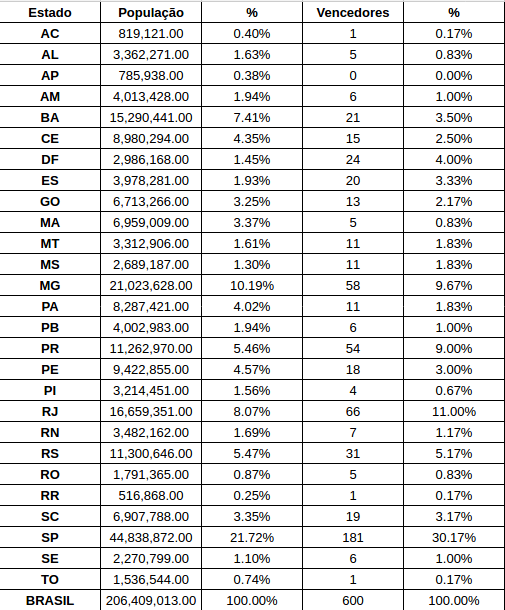
\includegraphics[scale=0.5]{table1}

Vemos na tabela que proporção tende a ser bastante semelhante, sugerindo a corretude estatística do concurso.

\subsection{Resultados por Valor Recebido pelos Vencedores}
Nesta tarefa, foram gastos 5 minutos e 31 segundos para a execução do \textit{mapper} e do \textit{reducer} pelo \textit{Hadoop}. Tempo também bastante viável. Veja os resultados obtidos na tabela a seguir.

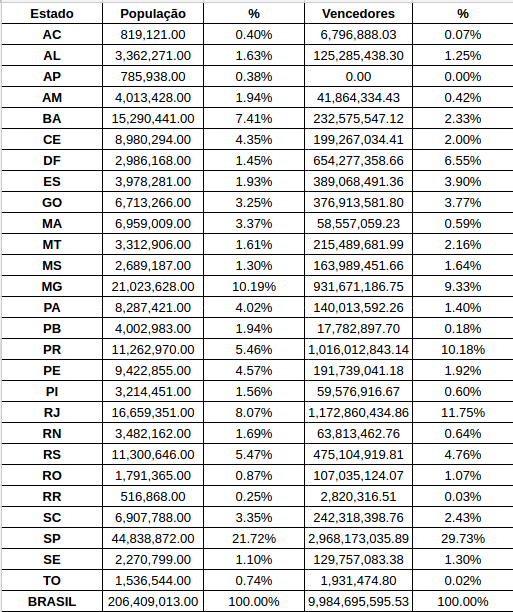
\includegraphics[scale=0.5]{table2}

Nesta tabela também podemos perceber certa tendência das proporções a seguirem a proporção da população. É verdade que neste caso a correlação está um pouco pior do que o visto pela primeira tabela, mas ainda assim sugere a corretude estatística do concurso.

%%%%%%%%%%%%%%%%%%%%%%%%%%%%%%%%%%%%%%%%%%%%%%%%%%%%%%%%%%%%%%%%%%%%%%%%%%%%%%%%%%%%%%%%%%%%%%%%%%%%%%%%%%%%%%%%%%%%%%%%%%%%%%%%%%%%%%%%%%%%%

\section{Conclusões}
Podemos concluir a partir dos resultados obtidos que o \textit{Hadoop} se mostra uma ferramenta bastante eficiente, somada ao paradigma de \textit{MapReduce} eles conseguem resolver problemas envolvendo grandes conjuntos de dados em tempo viável, o que seria impossível com ferramentas e paradigmas ordinários.

Sobre o concurso da Mega-Sena, fica difícil tirar muitas conclusões apenas com os dados coletados, principalmente por não estarmos usando a proporção de apostas, e sim a da população. Seria preciso um estudo mais aprofundado no assunto, com várias outras abordagens.

Mas para esse trabalho vimos que a proporção tende a ser semelhante à proporção da população dos estados, o que indicaria uma certa confiança no concurso, pois de certa forma mostra que não há tratamento preferencial para nenhum estado. Por outro lado, os mais céticos diriam que o concurso é manipulado para que os resultados se matenham numa proporção parecida com a proporção da população para que ninguém desconfie do concurso, porém, não podemos provar nada.

%%%%%%%%%%%%%%%%%%%%%%%%%%%%%%%%%%%%%%%%%%%%%%%%%%%%%%%%%%%%%%%%%%%%%%%%%%%%%%%%%%%%%%%%%%%%%%%%%%%%%%%%%%%%%%%%%%%%%%%%%%%%%%%%%%%%%%%%%%%%%

\begin{thebibliography}{9}
\bibitem{megasena} Resultados da Mega-Sena,\\
\texttt{http://loterias.caixa.gov.br/wps/portal/loterias/landing/megasena/}\\
(visitado em 13/09/2016)

\bibitem{udacity} Sarah Sproehnle, Ian Wrigley, and Gundega Dekena.\\
\texttt{https://udacity.com/course/intro-to-hadoop-and-mapreduce--ud617},\\
Intro to Hadoop and MapReduce, How to Process Big Data

\bibitem{github} Emerson Jair's Github,\\
\texttt{https://github.com/dungahk/mega-sena-hadoop}

\bibitem{ibge} Projeção da população do Brasil e das Unidades da Federação,\\
\texttt{http://www.ibge.gov.br/apps/populacao/projecao/}\\
(visitado em 14/09/2016 às 22:40)

\end{thebibliography}

\end{document}
